\documentclass[letterpaper]{article}
\usepackage[draft]{aaai2027}
\usepackage[hyphens]{url}
\usepackage{graphicx}
\urlstyle{rm}
\def\UrlFont{\rm}
\usepackage{natbib}
\usepackage{caption}
\usepackage{amsmath}
\usepackage{amssymb}
\usepackage{booktabs}
\frenchspacing
\pdfinfo{/TemplateVersion (2027.1)}
\setcounter{secnumdepth}{2}
\title{Graph-Conditioned Kernel Message Passing over Tree Sequences}
\author{Anonymous Submission}
\affiliations{}
\begin{document}
\maketitle
\begin{abstract}
Marginal genealogies combine changing anonymous ancestors with persistent sampled individuals. We develop a graph neural construction that reduces each observed tree to its sampled electrical interface, then repeatedly exchanges query context through graph-conditioned kernels at fixed genomic anchors. Integrated age potentials supply a small geometry bank while preserving serial subdivision. Exact finite anchor actions follow the true interval order and admit a positive semidefinite kernel interpretation, including noncommuting operators. Reference-inclusive row normalization bounds every kernel message. The construction preserves predictions under redundant graph-record subdivision and anonymous serial insertion with invariant observed leaf features. Matched controls separate age geometry, kernel depth, query coupling and positive-rate optimization. This working methods document accompanies ongoing validation-only architecture comparisons.
\end{abstract}

\section{Problem and Related Work}
We observe graphs $G_g$ on a partition of a continuous domain into intervals $I_g=[a_g,b_g)$. A persistent interface $S$ is present in every graph. Other vertices are graph-local. Predictions address query vertices $Q\subseteq S$ at fixed coordinates $x_p$. Observed reference vertices $R=S\setminus Q$ can carry labeled panel information. Numerical identifiers define correspondence only.

For ancestral recombination graphs, the domain is genomic position, each $G_g$ is a marginal genealogy, and $S$ contains sampled haplotypes. Query local ancestry is an external supervised target. Labeled reference samples, observed ages and reconstructed topology provide input evidence. ARGformer motivates inference from ARGs \citep{argformer2026}. Graph-transformer ancestry inference supplies a related task \citep{ancientancestry2026}, with broader biological context from ancient Eurasian ancestry \citep{eurasians2024}.

Graph Set Transformer interleaves graph processing and set attention \citep{gst2026}. GraphSSM studies continuous graph dynamics and persistent-node alignment \citep{graphssm2024}. Message-Passing State-Space Models propagate persistent hidden states through graph shift operators \citep{mpssm2026}. Kron reduction preserves a graph's static boundary response \citep{kron2013}, and Node Decimation Pooling already uses this reduction within GNN representation learning \citep{ndp2022}. Graph kernels derived from stochastic differential equations model nonseparable space-time covariance \citep{graphspde2022}. Kernel reconstruction also addresses space-time signals on dynamic graphs \citep{dynamicgraphkernel2017}. Our candidate combines a fixed sample interface with changing boundary operators and exact genomic-duration processing. The evaluation asks whether that combination supplies useful memory beyond these established components.

\section{Boundary Graph Construction}
\subsection{Observed Resistance and Reduction}
For a tree edge joining observed ages $t_u<t_v$, let its resistance be $r_{uv}=\kappa(t_v-t_u)$ for fixed $\kappa>0$. Ages are decoded before subtracting them. Assume every edge has positive resistance and every connected component containing an interior vertex touches the interface. The undirected conductance Laplacian is $L_g$. Partition its vertices into $S$ and anonymous interior $A_g$. The boundary response is
\begin{equation}
 C_g=(L_g)_{SS}-(L_g)_{SA}(L_g)_{AA}^{-1}(L_g)_{AS}.
\end{equation}
A linear solve implements the Schur complement. $C_g$ is symmetric positive semidefinite with zero row sums and nonpositive off-diagonal entries. With $y(v,u)=(v^\top,u^\top)^\top$, its energy characterization is
\begin{equation}
 v^\top C_gv=\min_u y(v,u)^\top L_g y(v,u).
\end{equation}
These are established Kron properties \citep{kron2013}.

Define $\bar C_g=C_g/s_g$, where $s_g$ is the mean boundary diagonal. A zero response uses $s_g=1$. This scalar normalization respects boundary permutation and serial-edge equivalence. It expresses coupling on a common dimensionless scale. Observed age summaries remain available to the encoder.

\subsection{Invariant Source Encoding}
The leaf feature bank $X_g^S$ contains observed sample roles, ages and fixed reference-relation summaries. The summaries use source-conditioned observed common-ancestor times, reference fractions, nearest-reference tie votes and fixed kernel evidence. They are precomputed independently within each observed tree. The raw parent-branch feature is excluded, since inserting a unary ancestor changes that feature at its child.

A graph-local GNN encodes $(X_g^S,\bar C_g)$ into $H_g$. Its conductance adjacency is $-\bar C_{g,ij}$ off the diagonal. Each residual layer uses a weighted neighbor mean, a learned self update and layer normalization. It receives no temporal state, coordinate or numerical-ID embedding. Shared projections produce bounded signals
\begin{align}
 F_g^Q&=\tanh(H_g^QW_Q^\top+b_Q),\\
 U_g^R&=\tanh(H_g^RW_R^\top+b_R).
\end{align}
Reference signals depend on observed panel information. The query ancestry target remains outside this source bank.


\subsection{Integrated Age Geometry}
Older genealogy branches can transmit evidence across populations that are distinct at the ancestry horizon. We therefore prepare a fixed positive resistance family from observed endpoint ages. For scales $s\in\{350,1400\}$ generations define
\begin{align}
 w_s(t)&=1+3t^2/(s^2+t^2),\\
 \Phi_s(t)&=4t-3s\arctan(t/s),\\
 r_{uv}^{(s)}&=\kappa[\Phi_s(t_v)-\Phi_s(t_u)].
\end{align}
The plain branch has $\Phi_0(t)=t$. A common plain scale $\sigma_g=\operatorname{mean}\operatorname{diag}(C_{g,0})$ normalizes every age response, $\widehat C_{g,s}=C_{g,s}/\sigma_g$. Consequently age attenuation is retained. A plain zero response uses $\sigma_g=1$.

Since $1\leq w_s\leq4$, conductance energies and their interior minima give
\begin{equation}
 \tfrac14 C_{g,0}\preceq C_{g,s}\preceq C_{g,0}.
\end{equation}
Endpoint potentials telescope under serial subdivision. Thus each age response and the common normalization preserve the same electrical equivalence contract as plain geometry.

The matched scalar-age control sets
\begin{equation}
 \widehat C^{\mathrm{scalar}}_{g,s}
 =\frac{\operatorname{mean}\operatorname{diag}(C_{g,s})}{\sigma_g}
 \widehat C_{g,0}.
\end{equation}
It retains age-dependent global attenuation while preserving the plain operator's relative geometry. The source encoder always uses the plain response and identical observed leaf features.


\section{Fixed-Anchor Kernel Message Passing}
\subsection{Conditional Graph Kernels}
For layer $\ell$, branch $s$ and latent channel $h$, global positive rates define
\begin{equation}
 K_{\ell,s,h}(x)=
 \lambda_{\ell,s,h}\widehat C_{g(x),s,QQ}
 +\delta_{\ell,s,h}I.
\end{equation}
Let $T_{\ell,s,h}(x,y)$ be its time-ordered homogeneous propagator for $x\geq y$. The symmetric matrix-valued kernel is
\begin{equation}
 \mathcal H_{\ell,s,h}(x,y)=
 \begin{cases}
 T_{\ell,s,h}(x,y),&x\geq y,\\
 T_{\ell,s,h}(y,x)^\top,&x<y.
 \end{cases}
\end{equation}
Each branch has a separate propagation state. Nonnegative global mixture weights are $\pi_{\ell,s,h}=\operatorname{softmax}_s(\alpha_{\ell,s,h})$. Mixing completed kernel actions preserves the branch-specific cached bases.

Every query eigensystem is fixed offline. On a hold of length $\Delta$, its action is
\begin{equation}
 Tz=V_{g,s}\operatorname{diag}
 \big(e^{-\Delta(\lambda_{\ell,s,h}\mu_{g,s}+\delta_{\ell,s,h})}\big)
 V_{g,s}^\top z.
\end{equation}
Products follow the observed interval order, including partial holds. This computation differentiates scalar rates and source projections while reusing fixed geometry.

\subsection{Physical Anchor Sources}
Choose $A=32$ equal-width cell midpoints $y_a$ on each supplied tile, with cell-width masses $\omega_a$. Anchors depend on physical endpoints and resolution. The graph-local GNN supplies query embeddings $U^0_{Q,a}$ and observed reference embeddings $U^0_{R,a}$ at the containing graph.

At layer $\ell$, bounded shared projections produce
\begin{align}
 q_{\ell,h,a}&=\tanh(W_{\ell,Q}U^\ell_{Q,a}+b_{\ell,Q})_h,\\
 r_{\ell,h,a}&=\tanh(W_{\ell,R}U^0_{R,a}+b_{\ell,R})_h.
\end{align}
The query source for branch $s$ is
\begin{equation}
 S_{\ell,s,h,a}
 =q_{\ell,h,a}
 -\lambda_{\ell,s,h}\widehat C_{g(y_a),s,QR}r_{\ell,h,a}.
\end{equation}
Reference embeddings remain graph-local observed sources throughout kernel depth. Query context is updated successively at fixed anchors.

For any anchor or requested readout $x$, the numerator is
\begin{equation}
 N_{\ell,h}(x)=
 \sum_s\pi_{\ell,s,h}\sum_a\omega_a
 \mathcal H_{\ell,s,h}(x,y_a)S_{\ell,s,h,a}.
\end{equation}
Run the same action on the matching ones source
\begin{equation}
 m_{\ell,s,h,a}=
 \mathbf1_Q-\lambda_{\ell,s,h}
 \widehat C_{g(y_a),s,QR}\mathbf1_R
\end{equation}
to obtain $D_{\ell,h}(x)$, and normalize elementwise as $M_{\ell,h}(x)=N_{\ell,h}(x)/D_{\ell,h}(x)$.

The gated residual update is
\begin{align}
 g_\ell(U,M)&=\operatorname{sigmoid}
 \big(W_{\ell,g}[U,M]+b_{\ell,g}\big),\\
 V_\ell(x)&=U^\ell(x)+g_\ell(x)\odot W_{\ell,M}M_\ell(x),\\
 U^{\ell+1}(x)&=\operatorname{LayerNorm}(V_\ell(x)).
\end{align}
Here $g_\ell(x)=g_\ell(U^\ell(x),M_\ell(x))$. Apply this update at anchors and requested coordinates. Only anchor embeddings create subsequent sources. The final shared linear head predicts from the updated readout embedding.

\subsection{Exact Finite Kernel Actions}
For one branch/channel, an inclusive forward sum and exclusive reverse sum give
\begin{align}
 a_p&=T(y_p,y_{p-1})a_{p-1}+\omega_pS_p,\\
 b_p&=T(y_{p+1},y_p)^\top(b_{p+1}+\omega_{p+1}S_{p+1}).
\end{align}
The message is $a_p+b_p$, with zero exterior states. Its self term appears once. Additional event coordinates evaluate arbitrary readouts using partial homogeneous actions without creating new impulses. Numerator and denominator share one bundled scan.

This is an exact action for the predeclared finite anchor measure. With $E$ physical subholds, its dense spectral propagation cost is $O(LESQ^2H)$ for kernel depth $L$, $S$ branches and $H$ latent channels. Source construction additionally costs $O(LASQRH)$. The graph encoder and CPU Schur/eigensystem preparation are separate measured costs.


\section{Kernel and Representation Properties}
\subsection{Positivity and Bounded Messages}
\textbf{Proposition 1.}
For symmetric positive definite piecewise-constant $K(x)$, the completed kernel $\mathcal H$ is positive semidefinite, including noncommuting holds. Global nonnegative mixtures preserve this property.

\textbf{Proof.}
Consider $dZ=-K(x)Z\,dx+\sqrt{2K(x)}\,dW$ with initial covariance $I$, independent of later Brownian increments. Its covariance equation is $P'=-KP-PK+2K$, with solution $P=I$. Cross-covariance is $T(x,y)$ for $x\geq y$, with the transpose in the opposite order. A covariance kernel is positive semidefinite, as is a nonnegative sum of such kernels. $\square$

This certificate uses established linear-process covariance theory \citep{sdes2019}. The conditional kernel acts on coordinates and persistent query samples within one observed collection.

\textbf{Proposition 2.}
For finite positive rates and positive anchor masses, each reference-inclusive normalized message is an elementwise convex combination of bounded query/reference source signals. In exact arithmetic, $|M_{\ell,h,q}(x)|\leq1$.

\textbf{Proof.}
The conductance response has nonpositive off-diagonal entries, so $-K$ is Metzler. Each local exponential is entrywise nonnegative, as are products and their transposes. Also $-\lambda C_{QR}\geq0$. Thus the expanded numerator has nonnegative coefficients on every anchored query and reference signal. The ones-source scan sums exactly those coefficients, producing a strictly positive denominator for finite rates and positive masses. Division gives a convex combination of signals in $[-1,1]$. $\square$

The normalized action has this bounded aggregation property. Its underlying symmetric kernel supplies the PSD statement. Finite arithmetic explicitly rejects nonpositive or nonfinite mass rather than adding an unreported denominator floor.

\subsection{Dual Subdivision Contract}
\textbf{Proposition 3.}
Under exact arithmetic and deterministic evaluation, predictions are preserved by splitting an unchanged graph interval into identical consecutive pieces, or by inserting anonymous serial vertices with preserved endpoint ages. The contract holds at every kernel depth when tile endpoints, physical anchors, interface partition, requested coordinates and invariant observed leaf features are fixed.

\textbf{Proof.}
Serial potential differences telescope, so electrical series equivalence preserves every response and the common plain normalization. The shared graph-local encoder therefore produces identical observed interface embeddings. Splitting an unchanged hold preserves each homogeneous propagator by the semigroup identity. Fixed anchors, their containing observed graph, and source masses remain identical. The first-layer numerator, denominator and updates are unchanged. Induction preserves all subsequent anchor sources and readout updates. $\square$

The 47-feature ancestry bank excludes raw immediate-parent branch length. Persistent numerical IDs serve correspondence only. Requested outputs never become source anchors, so adding readout coordinates leaves existing predictions unchanged. Implementation checks cover both subdivision operations, permutation, dense noncommuting propagators, self counting, gradients and numerical mass behavior.


\begin{figure*}[t]
\centering
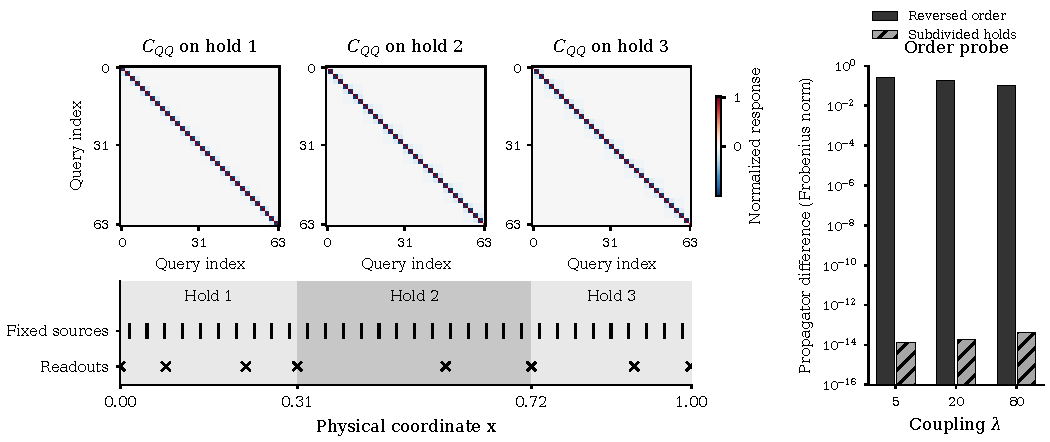
\includegraphics[width=\textwidth]{figures/operator_order_probe_v1.pdf}
\caption{Structural illustration from an untrained synthetic sequence with 64 query and 24 reference samples. Left: query boundary responses on three holds, with 32 fixed source anchors and independent readout coordinates. Right: Frobenius differences from the original ordered propagator at damping $\delta=1$. Reversing the same operator-duration pairs changes the action. Splitting each hold into three equal subholds preserves it to floating-point precision. This probe illustrates operator order and the semigroup property.}
\label{fig:operator-order}
\end{figure*}

The recorded synthetic probe in Figure~\ref{fig:operator-order} isolates homogeneous propagation. At coupling rates $\lambda=5,20,80$, reversing three observed holds gives Frobenius differences $0.278$, $0.185$ and $0.109$. Triple subdivision gives differences below $4.1\times10^{-14}$ in float64. The probe uses fixed geometry without neural fitting.

\section{Matched Evaluation Protocol}
\subsection{Attribution Controls}
All anchor comparisons share observed leaf features, the plain local encoder, fixed physical anchor measure, correspondence and readout coordinates. A factorial design contrasts one versus two kernel layers, plain versus age versus matched scalar-age geometry, and full versus scalar propagation.

The scalar propagation control replaces $C_{QQ}$ by $I$ only inside $K$, giving $K=(\lambda+\delta)I$. It preserves the original reference source map, learned projections, mixture weights and denominator definition. The local source encoder still combines spatial evidence. This ordinary temporal-kernel comparison changes both diagonal decay and spatial coupling. A raw diagonal control instead retains the full generator diagonal. A gain-matched diagonal control additionally transforms each numerator and ones source by $D K^{-1}$, where $D=\operatorname{diag}(K)$. This preserves homogeneous continuous-forcing DC gain while removing transfer between previous query states.

The three-branch plain control repeats the plain operator with the same initial rate schedule $(5,20,80)$ as the age branches. Full/scalar geometry comparisons have identical parameter schemas. Kernel depth changes parameter counts, which are recorded. Matched log-positive and softplus-positive rates have identical initial rates and parameters. Rate and mixture parameters receive zero weight decay in every anchor comparison.

Separate earlier boundary controls include graph-local prediction, scalar smoothing, recurrent and attention aggregation, homogeneous bags and matched-gain independent memory. Graph Set Transformer, GraphSSM and ARGMix paper-equation adaptations supply complementary architectural baselines with their input and reproduction scopes recorded.

\subsection{Biological Local Ancestry Study}
The biological development condition follows the eleven-population ancient-European simulation formulation of \citet{eurasians2024}. It retains four source populations and the BAA admixture path. Backward admixture events occur at 166 generations for Bronze ancestry from Neo and Yam, 259 for Neo ancestry from WHG and Ana, 177 for Yam ancestry from CHG and EHG, and 169 for BAA ancestry from CHG and Ana. Source fractions are respectively $(0.5,0.5)$, $(0.25,0.75)$, $(0.5,0.5)$ and $(0.25,0.75)$.

The target is the population occupied by a query lineage at census 350 generations, mapped to ANA, CHG, WHG and EHG. All scored queries are younger than that census. Pure-source reference dates are heterogeneous, and some references are older than the census. The reference population label describes observed panel membership rather than an additional query target.

Four independent 2 Mb simulations provide two training and two development-validation parents, using mutation rate $1.25\times10^{-8}$ and uniform recombination rate $10^{-8}$ per base per generation. Each parent contains 140 diploid individuals. The 280 haplotypes comprise 96 pure-source references, with 24 per source, 64 unlabeled admixed context haplotypes, and 120 query haplotypes. Queries comprise 64 present-day and 56 ancient haplotypes. This scaled panel is a declared task transfer from the original study.

Inference and prediction consume phased genotypes and observed sample metadata. Census annotations, ancestral populations and true ancestry boundaries remain outside the observation pipeline. The post-population-size Relate observations retain 955, 897, 946 and 920 marginal trees for the four parents. Eight physical 250 kb tiles per parent retain every marginal tree and all 280 sampled haplotypes. Electrical reduction uses every connected internal node and edge before producing the sampled interface.

The model uses 47 observation-only leaf features and whole-tree boundary operators. Its dynamic query interface has 184 haplotypes, consisting of the 120 scored queries and 64 unlabeled context haplotypes. Pure-source references form a separate 96-haplotype source interface. Only the actual 120 query outputs receive supervised loss or ancestry scoring. Integer sample IDs establish correspondence without learned ID embeddings.

The released AncestralPaths Dense model retains its native $5\times9$ cohort-shell features and six path probabilities. The common four-source readout sums the Ana and CHG probabilities across their direct and via-BAA paths before taking the argmax. ARGMix is evaluated using the pinned current author release, including its native transformer, recurrent refinement, reference selection and overlap probability averaging. ARGformer's released encoder, tokenizer and pooler use within-genealogy unsupervised path learning and pure-reference contrastive labels. This transductive setting is distinguished from supervised transfer across simulated parents. Its published tsinfer plus tsdate inference family provides shared ancestral tokens. Representation qualification therefore precedes interpretation of a transfer to a different inferred genealogy. Each baseline is identified by its inference pipeline, native implementation and explicit task adaptations.

Earlier engineering cohorts use the pinned stdpopsim 0.3.0 \texttt{AncientEurope\_4A21} model with eight or 64 query haplotypes. Their exploratory outcomes remain separate from the biological development condition.

The paired Relate 1.2.4 pipeline uses observed phased variants, sample ages and a declared recombination map. Its genuine SNP coverage clips edge tiles without chromosome-tail extrapolation. Exact original 100 bp grid centers and query identities are retained. Scoring intersects clipped physical bins with full truth spans. Relate attribution: Copyright \copyright\ 2018, University of Oxford.

Independent simulation parents are split before constructing eight fixed windows. The candidate and reconstructed architectural controls select checkpoints by minimum mean parent-validation negative log likelihood. Native baseline fitting and checkpoint selection follow their released implementations. Dataset, parent, preparation, code and prediction hashes bind each comparison. Records retain accuracy, NLL, calibration diagnostics, parameter count, preparation cost, training time and GPU memory. Exploratory cohorts contain training and validation data only.


\subsection{Biological Development Observations}
\begin{table}[t]
\centering
\caption{Development observations on the same two validation parents and exact present-day query support. Fits counts optimizer seeds. Native ARGformer uses tsinfer/tsdate and per-ARG transductive learning. The last three rows refine frozen ARGMix. Their reference refinements use independent tsinfer context.}
\label{tab:biological-development}
\begin{tabular}{lrrr}
\toprule
Method & Fits & Acc. (\%) & NLL \\
\midrule
Current ARGMix & 1 & 85.55 & 0.435 \\
Candidate age D2 & 3 & 84.78 & 0.430 \\
Candidate plain D2 & 3 & 84.79 & 0.430 \\
Matched GRU D2 & 3 & 84.07 & 0.454 \\
AncestralPaths Dense & 3 & 82.06 & 0.819$^{*}$ \\
GST-style 32 & 1 & 80.03 & 0.569 \\
GST-style 64 & 1 & 79.86 & 0.569 \\
Native ARGformer top1 & 1 & 75.68 & $\infty$ \\
ARGMix plus smoothing & 1 & 85.94 & 0.389 \\
Reference context & 1 & 85.91 & 0.382 \\
Ancestral traces & 1 & 85.93 & 0.383 \\
\bottomrule
\end{tabular}
\par\smallskip
\parbox{\columnwidth}{\footnotesize $^{*}$Auxiliary NLL uses native logits with stable log-sum-exp. Weights and ancestry argmax are unchanged. Original softmax underflow remains recorded. ARGformer hard votes retain zero true-class probabilities. No probability floor is applied. These are adapted development tasks, not original-paper numerical reproductions.}
\end{table}

Table~\ref{tab:biological-development} reports completed fits on the biological development condition. The age candidate averages 84.78\% present-day accuracy across three optimizer seeds, compared with 82.06\% for released AncestralPaths Dense and 80.03\% for the width-32 GST-style control. Current ARGMix reaches 85.55\%. The age candidate has slightly lower NLL and higher Brier error than ARGMix. Age and plain candidates differ by only 0.01 accuracy points. These observations do not establish an age-conditioning advantage or overall superiority.

The ARGMix row uses the current author release with native fitting, selection, refinement and overlap averaging. AncestralPaths retains its released Dense architecture, native features, six-path outputs and the declared common-source readout. GST rows are independently reconstructed architectural controls. Native ARGformer retains the author encoder, objectives, full batches and exhaustive reference retrieval. Each observed ARG receives five masked-language-model epochs and one contrastive epoch without query ancestry labels. Top1 ancestry accuracy is 75.68\%, with a prespecified top5 sensitivity of 75.14\%. Its inferred tsinfer/tsdate genealogy and transductive objective differ from the supervised Relate pipeline, so this is a descriptive common-endpoint transfer comparison.

A separate FP32 discovery experiment uses frozen ARGMix emissions with independent tsinfer whole-tree geometry. Ordinary genomic smoothing improves accuracy to 85.94\% and NLL to 0.389. Native-age reference context reduces NLL further to 0.382 while accuracy is 85.91\%. Census-conditioned affinity does not improve on its age-free control. Reference-only genuine ancestral propagation reaches 85.93\% and NLL 0.383, essentially matching sample-only propagation. A shuffled ancestral-history control reaches 86.04\% with worse NLL and substantially more spurious tract boundaries. It provides no evidence for a genuine ancestral-continuity advantage. The frozen smoother was selected on development data and TRAIN emitter predictions are in-sample.

The independent biological unit is the simulation parent. All observations reuse two development parents, with no TEST evaluation. Seed means describe separate fits rather than probability ensembles, and optimizer seeds are not independent biological replicates. The discovery controls use one FP32 seed and 160 updates per arm, selected by minimum equal-parent present-day NLL. The results motivate further architecture development but do not establish distinct GNN novelty, original-paper numerical reproduction or independent biological generality.

The Hungarian Chickenpox Cases dataset supplies an external chronological forecasting setting on a persistent 20-county graph. It has 522 observations and a CC BY 4.0 license. Inputs contain 52 historical weeks and predict the following week. The chronological split has 313 training targets, 78 validation targets and 79 reserved test targets. Normalization uses training observations only. Seasonal, persistence and multivariate ridge controls accompany neural comparisons. Graph SPDE kernels also evaluate on this dataset \citep{graphspde2022}, motivating a covariance-based comparator. This fixed-topology setting evaluates temporal applicability alongside the changing-tree ancestry study.

\bibliography{references}
\end{document}
